% PHYSICS OF FLUIDS
%\documentclass[aip, pof, reprint]{revtex4-1} 
% the files aip4-1.rtx seems to be necessary
%\documentclass[11pt]{article}

\documentclass[onecolumn,showpacs,preprintnumbers,amsmath,amssymb]{revtex4-2}

% PACKAGES
\usepackage{graphicx, amsmath, amssymb, amsfonts, mathtools, mathrsfs, color}
\usepackage{natbib, comment, todonotes}
\usepackage[justification=RaggedRight]{caption}
% Unneeded?
%\usepackage{subfig, wrapfig, bbm} 
\usepackage[margin = 1.5cm]{geometry} % Changes margins
\usepackage{xcolor}
\usepackage[capitalise]{cleveref}
%---------------------------------------------------------------------------%
% COMMANDS

% Basic editing
\newcommand{\nick}[1]{{\color{orange}#1}}
\newcommand{\tocite}{{\color{blue}(to cite)}}
\newcommand{\vsp}[1]{\vspace{#1 pc} \noindent}
\newcommand{\np}{\newpage \noindent}
% Basic math, derivatives
\newcommand{\td}[2]{\frac{d #1 }{d #2}}
\newcommand{\ttd}[2]{\frac{d^2 #1 }{{d #2}^2}}
\newcommand{\pd}[2]{ \frac{ \partial #1}{ \partial #2 } }
\newcommand{\ppd}[2]{ \frac{ \partial^2 #1}{ {\partial #2}^2 } }
\newcommand{\pdi}[2]{ { \partial #1} / { \partial #2 } }
% Basic math, vectors and other
\newcommand{\bvec}[1]{{\mathbf{#1}}}
%\newcommand{\bvec}[1]{\ensuremath{\boldsymbol{#1}}}

\newcommand{\grad}{\nabla} 
\newcommand{\abs}[1]{\left| #1 \right|}
\newcommand{\norm}[1]{ \left\| #1 \right\| }
\newcommand{\ip}[1]{ \langle #1 \rangle }
\newcommand{\mean}[1]{ \langle #1 \rangle}
% For real and imaginary, could use \Re or \Im, or \mathcal{R}, or \text{Re}
\newcommand{\Lap}{\grad^2}
\newcommand{\real}{\operatorname{Re}}
\newcommand{\imag}{\operatorname{Im}}

\newcommand{\vd}[2]{\frac{\delta #1 }{\delta #2}}
\newcommand{\Vol}{\text{Vol}(\Omega)}

\newcommand{\uu}{\bvec{u}}
\newcommand{\uopt}{\uu_{\text{opt}}}
\newcommand{\vv}{\bvec{v}}
\newcommand{\xx}{\bvec{x}}

\newcommand{\Bvec}{\bvec{B}}
\newcommand{\Bhat}{\hat{\Bvec}}
\newcommand{\jvec}{\bvec{j}}

\newcommand{\weight}{w}
\newcommand{\Lmult}{\lambda}

\newcommand{\ex}{\hat{\bvec{e}}_1}
\newcommand{\ey}{\hat{\bvec{e}}_2}


\newcommand{\proj}{ \mathcal{P}_{\text{df}} }
\newcommand{\phat}{ \hat{\mathcal{P}}_{\text{df}} }
\newcommand{\nproj}{ \bar{\mathcal{P}}_{\text{df}} }

\newcommand{\kk}{\bvec{k}}
\newcommand{\eikx}{e^{ i \left( k_1 x + k_2 y \right) }}
\newcommand{\vrand}{\vv_{\text{rand}}}


%\newcommand{\Mprod}{\mathcal{P}}
%\newcommand{\Mdiss}{\mathcal{D}}
%\newcommand{\growA}{\lambda_A}
%\newcommand{\growB}{\lambda_B}
%\newcommand{\obj}{\dot{E}_A}
%\newcommand{\const}{c}


% Dash integral
\def\Xint#1{\mathchoice
   {\XXint\displaystyle\textstyle{#1}}%
   {\XXint\textstyle\scriptstyle{#1}}%
   {\XXint\scriptstyle\scriptscriptstyle{#1}}%
   {\XXint\scriptscriptstyle\scriptscriptstyle{#1}}%
   \!\int}
\def\XXint#1#2#3{{\setbox0=\hbox{$#1{#2#3}{\int}$}
     \vcenter{\hbox{$#2#3$}}\kern-.5\wd0}}
\def\ddashint{\Xint=}
\def\dashint{\Xint-}


%---------------------------------------------------------------------------%
% DOCUMENT

\begin{document}

\title{Optimal velocity fields for instantaneous dynamo action}

%dynamo growth or dynamo action?
%\title{Dynamo-optimizing velocity fields}

%\author{Nicholas J.~Moore }
%\thanks{Colgate University} 
%\author{Stefan G.~Llewellyn Smith} 
%\thanks{Department of Mechanical and Aerospace Engineering, Jacobs School of Engineering, UCSD}
%\author{Keaton J.~Burns} 
%\thanks{Department of Mathematics, Massachusetts Institute of Technology, Cambridge MA 02139, USA }

\begin{abstract}
We consider a variant of the kinematic dynamo problem. Rather prescribing the velocity field and solving an eigenvalue problem to determine the magnetic field that exhibits maximal growth rate, we treat the seed magnetic-field structure as given and ask which velocity field maximally enhances its growth. We show this second problem has an elegant formulation in terms of variational calculus. Constraining a weighted sum of kinetic energy and enstrophy yields a forced Helmholtz equation with the Lorentz force acting as the inhomogeneity. For the special case of fixed kinetic energy, the problem can be solved exactly and the optimal velocity field everywhere opposes the divergence-free projection of the Lorentz force. Under more general constraints, the optimal velocity profile can differ from the Lorentz force field and can be found by solving the forced Helmholtz equation numerically. 
We demonstrate these results through 2.5-dimensional periodic examples.
\end{abstract}

%This result is consistent with direct inspection of the magnetic-energy law. 

\maketitle

%---------------------------------------------------------------------------%
\section{Introduction}
The flow of conducting fluids deep in the interiors of stars and planets creates large-scale magnetic fields through the dynamo mechanism \cite{Moffatt2019, Tobias2021}. A natural question is what types of flow fields can produce dynamo action and which flows are best at it? The classical kinematic dynamo problem addresses this question by prescribing a velocity field, most often steady in time, and formulating an eigenvalue problem to determine the magnetic-field growth rate \cite{Moffatt2019, Tobias2021}. The eigenfunction with the largest eigenvalue corresponds to the magnetic field that is maximally enhanced by the velocity field that was chosen.

A class of recent studies have extended the kinematic dynamo problem beyond the simple eigenvalue formulation. These studies apply variational calculus techniques to numerically optimize the velocity-field-magnetic-field pair for growth rate of the later \cite{Willis2012, Chen2015, Chen2018, Luo2020}. These studies have been conducted in a range of geometries. In these studies, though the velocity field is numerically optimized, it is still treated as specified. For example, it does not evolve according to any physical governing equations. 

We propose a new variant of the kinematic dynamo problem. In particular, we treat the seed magnetic field, rather than the velocity field, as the prescribed object. We then seek the companion velocity field that maximally enhances the instantaneous growth rate of this magnetic field. We find that this new variant has an elegant formulation in variational calculus, yielding a forced Helmholtz equation for the desired velocity field with the Lorentz force acting as the inhomogeneity. The problem can be constrained by fixing the budget of kinetic energy, enstrophy, or a linear combination of the two. For the case of fixed energy, the forced Helmholtz equation admits an exact solution and shows the optimal velocity field to everywhere oppose the divergence-free projection of the Lorentz force. For a combined constraint on energy and enstrophy, the forced Helmholtz equation can be solved numerically....

% FROM ABSTRACT: Constraining a weighted sum of kinetic energy and enstrophy yields a forced Helmholtz equation for the optimal velocity field with the Lorentz force acting as the inhomogeneity. 


\vsp{3}
Point to make: The problem studied here may constitute a first step towards inferring interior flow structures from surface magnetic field measurements. Detailed measurements of the surface magnetic field are practical whereas direct measurements of the flows of conducting fluid deep in the interior are less feasible.
While the detailed structure of the interior flow is not known, it must be of the variety to transfer considerable energy into the magnetic field and thus support it against against ohmic dissipation.
A natural starting point in the search of such fields is thus determining the flow field the maximizes the energy transferred to the magnetic field.

\vsp{3}
Another point: We demonstrate with 2.5 dimensional examples. Though they cannot be long-time dynamos, they exhibit strong instantaneous growth. These are only to illustrate the method in a simple way. Later work will consider fully 3D examples and search for long-time dynamos.


%---------------------------------------------------------------------------%
\section{Optimal velocity fields}

\subsection{Governing equations}

The solenoidal magnetic field $\Bvec$ evolves according to the induction equation \cite{Brandenburg1998, Glatzmaier1998, Willis2012, Yadav2016, Moffatt2019, Tobias2021}
\begin{align}
\label{induction}
\pd{}{t}  \Bvec &= \grad \times \left( \uu \times \Bvec \right) + \eta \grad^2 \Bvec  \, , \\
\label{solenoid}
\grad \cdot \Bvec &= 0
\end{align}
where $\eta$ is the magnetic diffusivity of the fluid. % Note: Brandenburg is the only one that calls eta the conductivity. All other sources call it the magnetic diffusivity so I should go with that.
Associated with the magnetic field is the current
\begin{align}
\label{j_defn}
\jvec = \mu_0^{-1} \grad \times \Bvec
\end{align}
where $\mu_0$ is the permeability. We usually non-dimensionalize by setting $\mu_0 = 1$. 

Consider the mean magnetic energy
\begin{equation}
M(t) = \frac{1}{2 \mu_0} \, \dashint_{\Omega} \abs{\Bvec}^2 \, dV \, .
\end{equation}
where the dashed integral indicates the mean value over  domain $\Omega$,
\begin{equation}
\dashint_{\Omega} \cdot  \,\, dV := \frac{1}{\Vol} \int_{\Omega} \cdot \,\, dV \, .
\end{equation}
%
The growth rate of magnetic energy is given by \cite{Tobias2021}
\begin{align}
\label{Mdot1}
\dot{M} = \mu_0^{-1} \, \dashint_{\Omega} \Bvec \cdot \Bvec_t \, dV 
& = \mu_0^{-1} \, \dashint_{\Omega} \Bvec \cdot \left( \grad \times \left( \uu \times \Bvec \right) + \eta \grad^2 \Bvec \right) \, dV \\
\label{Mdot2}
& = - \, \dashint_{\Omega} \uu \cdot \left( \jvec \times \Bvec \right) \, dV - \eta \mu_0 \dashint_{\Omega} \abs{\jvec}^2 \, dV
\end{align}
where the second line follows from integration by parts. 

% Mdot DECOMPOSITION
\begin{comment}
Prompted by the second line, we decompose $\dot{M}$ into the components
\begin{align}
\label{Mdot_decomp}
\dot{M} &= \Mprod - \Mdiss \, , \\
\label{Mprod}
\Mprod &= - \, \dashint_{\Omega} \uu \cdot \left( \jvec \times \Bvec \right) \, dV \, , \\
\label{Mdiss}
\Mdiss &= \eta \mu_0 \dashint_{\Omega} \abs{\jvec}^2 \, dV \, ,
\end{align}
Above $\Mprod$ represents the rate of production of magnetic energy by the velocity field $\uu$. This is the only term that can produce magnetic energy. $\Mdiss$ represents ohmic dissipation. This term is sign-definite and independent of the velocity field. 
%Since $\Mdiss$ is independent of $\uu$, the maximizer of $\Mprod$ also maximizes $\dot{M}$.
\end{comment}

Our goal is to maximize the instantaneous magnetic growth rate $\dot{M}$ over the space of permissible velocity fields. The incompressible velocity field, $\grad \cdot \uu = 0$, must be constrained in magnitude by either the energy or enstrophy, or some combination. The energy and enstrophy are respectively defined as
\begin{align}
\label{kinetic_energy}
E &= \frac{1}{2} \, \dashint \abs{\uu}^2 \, dV \, , \\
\label{enstrophy}
\mathcal{E} &= \frac{1}{2} \, \dashint_{\Omega} \abs{\grad \times \uu}^2 dV \, ,
\end{align}


%---------------------------------------------------------------------------%
\subsection{Optimization problem}

The optimization problem is as follows. For a prescribed seed magnetic field $\Bvec \vert_{t=0}$ with normalized magnetic energy $M(0)$, find the velocity field $\uu$ that instantaneously maximizes the quantity $\dot{M}$ from \cref{Mdot2}, subject to the constraints:
\begin{align}\
\label{div_free}
& \grad \cdot \uu = 0 \, , \\
\label{energy_enstrophy}
& \weight E + (1-\weight) \mathcal{E} = 1 \, ,
\end{align}
where $ 0 \le \weight \le 1$ represents the relative weight of energy versus enstrophy in the constraint. 

We solve the optimization problem by calculus of variations. 
For the divergence-free condition \cref{div_free}, we enforce the equivalent condition:
\begin{align}
\label{div_free_var}
\dashint_{\Omega} \Pi(\xx) \, \left(\grad \cdot \uu \right) \, dV = 0 \, ,
\end{align}
for any test function $\Pi(\xx)$. Integrating by parts shows that the operator in \cref{div_free_var} has variation derivative $-\grad \Pi$.
The optimal velocity field $\uu = \uopt$ satisfies the following Euler-Lagrange equation
\begin{equation}
\label{EulerLagrange}
\vd{\dot{M}}{\uu} - \grad \Pi + \Lmult \weight \vd{E}{\uu} + \Lmult (1-\weight) \vd{\mathcal{E}}{\uu}  = 0
\end{equation}
where $\Lmult$ is a Lagrangian multiplier that will be selected to enforce \cref{energy_enstrophy} and the function $\Pi(\xx)$ will be selected to enforce incompressibility \cref{div_free}.

Elementary calculations gives the following variational derivatives
\begin{align}
\vd{\dot{M}}{\uu} &= - \jvec \times \Bvec \, , \\
\vd{E}{\uu} &= \uu \, \, .
\end{align}
Taking the variational derivative of \cref{enstrophy} gives
\begin{align}
\delta \mathcal{E} 
&= \int_{\Omega} (\grad \times \uu) \cdot (\grad \times \delta \uu) \, dV \\
&= - \int_{\Omega} \grad^2 \uu \cdot \delta \uu \, dV - \int_{\partial \Omega} \left( \grad \times \uu \right) \times \delta \uu \, dS
\end{align}
We will work in a periodic domain, which allows us to drop the boundary integral above. In this case, rewriting the Euler-Lagrange \cref{EulerLagrange} with $C = -1/\Lmult$ gives
\begin{align}
\label{PDE1}
\weight \uu - (1-\weight) \grad^2 \uu = C \left( - \jvec \times \Bvec - \grad \Pi \right)
\end{align}
The function $\Pi(\xx)$ enforces the incompressible condition and the constant $C$ enforces the energy-enstrophy condition \cref{energy_enstrophy}. The above is a forced Helmholtz equation for the optimal $\uu$.
%elliptic partial differential equation (PDE) for the optimal $\uu$.

To simplify, we introduce a divergence-free projection operator $\proj$. That is, for any sufficiently smooth vector field $\vv$, let
\begin{align}
\label{div_free_project}
\proj[ \vv ] = \vv - \grad p \, ,  \text{  where } \grad^2 p = \grad \cdot \vv
\end{align}
It follows that $\grad \cdot \proj[ \vv ] = 0$ for any such field $\vv$.
Since the divergence commutes with the Laplacian,  the PDE for the optimal velocity field \cref{PDE1} can be rewritten as
\begin{align}
\label{PDE2}
\weight \uu - (1-\weight) \grad^2 \uu = C \, \proj \left[ - \jvec \times \Bvec \right]
\end{align}

The special case $\weight=1$ corresponds to a unit constraint on kinetic energy and no constraint on the enstrophy. In this case, the dynamo-optimizating velocity field is 
\begin{equation}
\uopt = C \, \proj \left[ - \jvec \times \Bvec \right] \, ,
\end{equation}
that is, the divergence-free projection of the negative Lorentz force. This result can perhaps be intuited by \cref{Mdot2}, where it is seen that to maximize $\dot{M}$ one maximizes the component of $\uu$ that aligns with the direction $- \jvec \times \Bvec$. As noted by Willis \cite{Willis2012}, the velocity gradient may be arbitrarily large in this special case which may be viewed as unphysical.
%
The opposite extreme of $\weight = 0$ corresponds to a unit constraint on enstrophy and no constraint on energy. In this case, $\uu = \uopt$ satisfies the Poisson equation
\begin{align}
\grad^2 \uu = C \, \proj \left[ \jvec \times \Bvec \right]
\end{align}


\vsp{5}

A huge benefit is that our results can narrow the search for optimal kinematic dynamos considerably. The kinematic dynamo problem consists of finding a velocity/magnetic field {\em pair} that leads to dynamo action. Thus, finding optimal dynamos requires searching a direct product of two function spaces (that for the velocity field and that for the magnetic field). Consider this problem approached numerically, where $O(N)$ grid points (or coefficients) are used to specify the velocity field and the magnetic field each. Then the optimization requires searching an $O(N^2)$ space. But the explicit formula () linking the velocity and magnetic field allows one to search only over the space of permissible magnetic fields (or maybe velocity fields) thus reducing the search to $O(N)$. In typically examples, $N$ might be on the order of 100, giving an increased efficiency of order 100.

\vsp{5}

%---------------------------------------------------------------------------%

\section{Numerical examples}

We now introduce some numerical examples to demonstrate that the solution of \cref{PDE2} gives the optimal growth of the the magnetic energy $M$ by comparing against randomly selected velocity fields.

\subsection{Numerics}

We aim to construct the simplest examples capable of dynamo action.
To this end, we work with three-dimensional vector fields depending on only two spatial variables in a periodic domain $(x,y) \in [0, 2\pi)^2$:
\begin{align}
\vv &= (v_1(x,y), v_2(x,y), v_3(x,y)) \, ,
\end{align}
often called 2.5-dimensional vector fields. We will consider all the velocity field $\uu$, the magnetic field $\Bvec$, and the current $\jvec$ each to be 2.5-dimensional fields.
Consider such a vector field with Fourier components up to cutoff wavenumber $K$
\begin{align}
\label{vec_Fourier}
\vv &= \sum_{k_1 = -K}^{K} \sum_{k_2 = -K}^{K} \hat{\vv}_{k_1, k_2} \, \eikx
\end{align}
The Fourier coefficients $\hat{\vv}_{k_1, k_2}$ are vector valued.

We first show how the divergence-free projection $\proj$ from \cref{div_free_project} is computed. The auxiliary scalar function $p$ satisfies $\grad^2 p = \grad \cdot \vv$ and so its Fourier coefficients are given by
\begin{align}
\label{}
\hat{p}_{k_1, k_2} = -i  \left( k_1 \ex + k_2 \ey \right) \cdot \hat{\vv}_{k_1,k_2} / k^2
\end{align}
where $\ex = (1,0,0)$ and $\ey = (0,1,0)$ and $k^2 = k_1^2 + k_2^2$. Let $\bvec{w} = \proj[ \vv ] = \vv - \grad p$. Then the Fourier coefficients of $\bvec{w}$ are given by
\begin{align}
\label{}
\hat{\bvec{w}}_{k_1, k_2} = \hat{\vv}_{k_1,k_2} - i \left( k_1 \ex + k_2 \ey \right) \hat{p}_{k_1,k_2}
\end{align}
and the field $\bvec{w}$ is guaranteed to be divergence free.

We next show how to compute the optimal velocity field through solution of the forced-Helmholtz equation \cref{PDE2}. If $\bvec{w} = \proj \left[ - \jvec \times \Bvec \right]$, then in Fourier space, an unnormalized solution of \cref{PDE2} is given by
\begin{align}
\label{PDE2}
\hat{\uu}_{k_1,k_2} = \frac{\hat{\bvec{w}}_{k_1,k_2} }{ \left( \weight + (1-\weight) (k_1^2 + k_2^2) \right)  }
\end{align}
We then simply normalize the solution to satisfy \cref{energy_enstrophy}.


\subsection{Numerics}

We begin with a magnetic field $\Bvec$ with a fixed spatial structure. We aim to use the simplest example field capable of dynamo action.
To this end, we work in the periodic cube $(x,y,z) \in [0, 2\pi)^3$ and assume the three-dimensional vector field $\Bvec$ depends  on $x$ and $y$ only. Since we allow three nontrivial components $\Bvec = (B_1, B_2, B_3)$ dynamo action is possible with no violation of the Cowling anti-dynamo theorems \cite{Moffatt2019}. We define the divergence-free magnetic field through its Fourier components 
\begin{align}
\label{B_Fourier}
\Bvec &= \nproj \left[ e^{i k z}
\sum_{k_1=0}^{K} \sum_{k_2=-K}^{K}
\hat{\Bvec}_{k_1, k_2} \, \eikx + c.c. \right]
\end{align}
where $\nproj$ represents the divergence-free projection operator normalized to give unit energy.
The above represents a Fourier series truncated at wavenumber $K$.

\nick{Note: Above is how I want to define the magnetic field so that (a) there is z-dependence and thus no Cowling gotchas, (b) the index range of $k_1$ and $k_2$ (along with the c.c.) takes care of the symmetries due to the field being real (and also so that the formula is consistent with my code)}.

To gain an understanding of the complexity of the magnetic fields generated for a particular $K$, it is beneficial to count the degrees of freedom. Given that the constant mode $\hat{\Bvec}_{0,0}$ has been removed, there are ostensibly $4K(K+1)$ non-zero, complex Fourier coefficients in \cref{B_Fourier}, where each coefficient $ \hat{\Bvec}_{k_1, k_2}$ is vector valued with three components. Because the field $\Bvec$ is real, the coefficients satisfy the conjugate relation $\hat{\Bvec}_{-k_1, -k_2} = \hat{\Bvec}_{k_1, k_2}^*$ and so there are $2K(K+1)$ independent, complex-vector coefficients. Since each coefficient is a vector of length three, there are $6K(K+1)$ complex-scalar degrees of freedom or $12K(K+1)$ real-scalar degrees of freedom.
The divergence-free constraint and the normalization each remove a degree of freedom. \nick{(I think the div-free here is a mistake; Div-free constraint removes more than a single constraint)}
Additionally, translations over the $xy$-plane removes two degrees of freedom, resulting in a total of $12K(K+1) - 4$ degrees of freedom. 
Thus, even a $K=1$ truncation corresponds to 20 real degrees of freedom in the magnetic field.

\nick{Calculation with Stefan on July 7, 2025. We calculated the degrees of freedom for the case $K=1$, for which $k=-1,0,1$. There is thus a $3\times3$ grid of ordered pairs, remove the $(0,0)$ mode gives 8 ordered pairs. There are three component of the B-field which gives 24 dof. The div-free constraint is a constraint for each ordered pair $(k_1,k_2)$ removing 8 dof. We now have a total of 16 dof. Normalization brings it to 15. Translations brings it to 13. So there are 13 real degrees of freedom. Note that the conjugate relation and the fact that a complex number is two real numbers balance each other out.}

\nick{For 3D, }
 
The optimal velocity field given by the solution to \cref{PDE2} is quadratic in $\Bvec$ (since $\jvec = \grad \times \Bvec$) and therefore will possess non-trivial Fourier components up to wavenumber $2K$. For a faithful comparison, we therefore consider randomly selected velocity fields with the same number of components
\begin{align}
\label{vrand}
\vrand &= \nproj \left[ 
\sum_{k_1=0}^{K} \sum_{k_2=-K}^{K}
\hat{\vv}_{k_1, k_2} \, \eikx + c.c. \right]
\end{align}
Similar to the magnetic field, we remove the constant mode $\hat{\vv}_{0,0} = 0$ \nick{(Can I justify this? See note in Codes Folder.)}, and since the velocity field is real, the conjugate relation is satisfied $\hat{\vv}_{-k_1, -k_2} = \hat{\vv}_{k_1, k_2}^*$. The number of degrees of freedom in $\vrand$ is $24K(2K+1) - 4$ (i.e.~the same as in $\Bvec$, just with $K$ replaced by $2K$).

\vsp{5}
TO DO
\begin{itemize}
\item Need to say how coefficients $\hat{\Bvec}$ are chosen. i.e. mean-zero Gaussian or perturbation of $\uopt$.
\item Need to give spectral algorithm for div-free projection $\proj$.
\end{itemize}


\begin{figure*}[htb]
\centering
 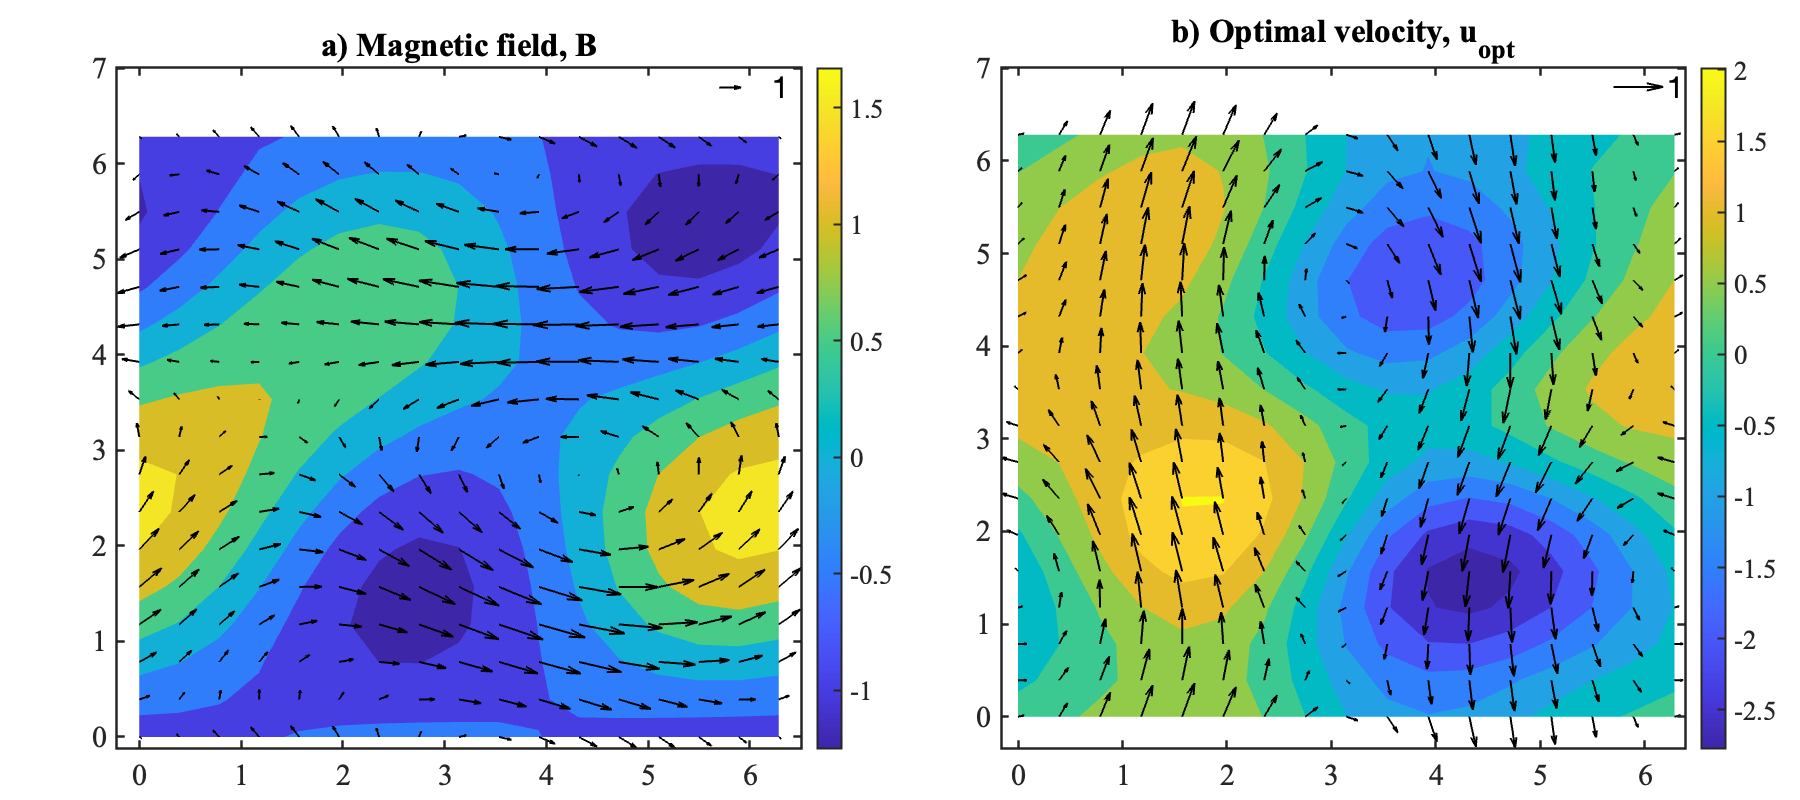
\includegraphics[width=.99 \linewidth]{vfields_ran_K=1.png}
 \caption{
a) $\Bvec$ is selected randomly.
b) The optimal velocity field that corresponds to the randomly selected $\Bvec$, giving $\dot{M} = 0.98$.}
\label{vfields_ran_K=1}
\end{figure*}
% N =16, K = 1, weight = 0.5

\begin{figure*}[htb]
\centering
 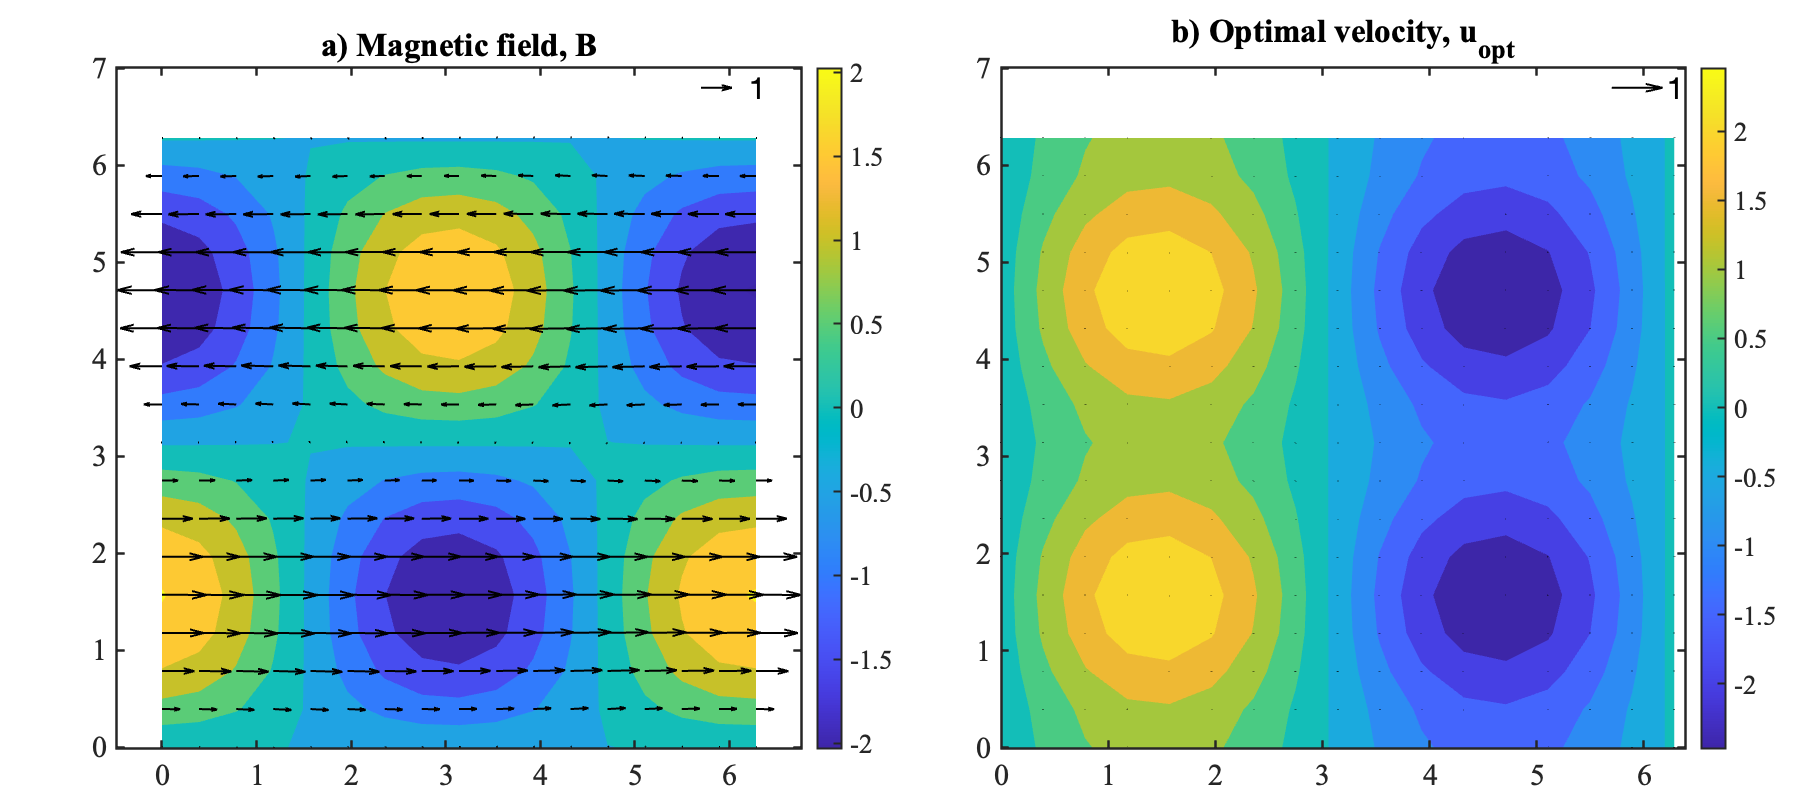
\includegraphics[width=.99 \linewidth]{vfields_opt_K=1.png}
 \caption{
a) $\Bvec$ is \nick{numerically?} optimized for maximal $\dot{M}$ (while using the corresponding $\uopt$ in each iteration of the optimization).
b) The optimal velocity field that corresponds to the optimized $\Bvec$, giving $\dot{M} = 1.53$.}
\label{vfields_opt_K=1}
\end{figure*}
% N =16, K = 1, weight = 0.5

\begin{figure*}[htb]
\centering
 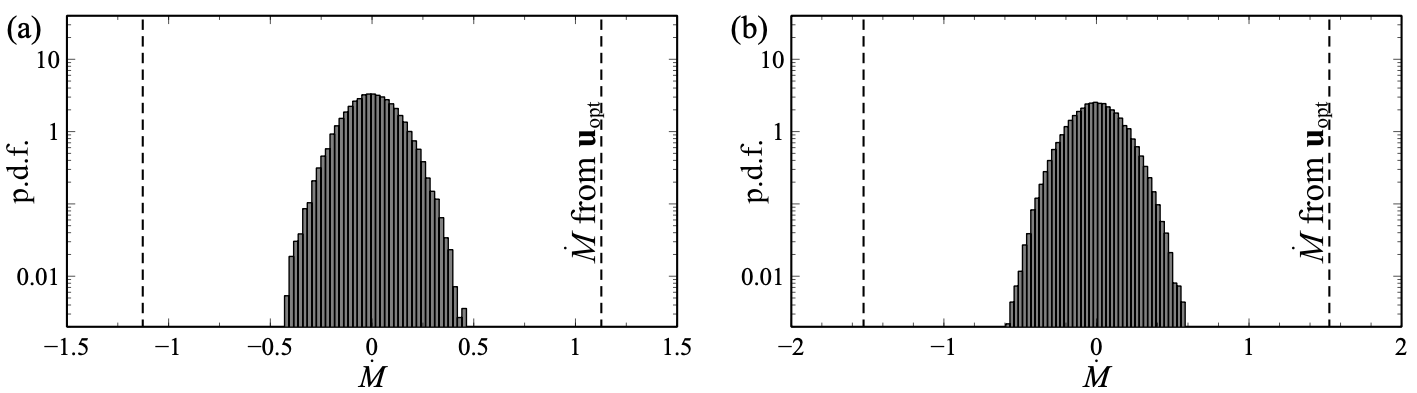
\includegraphics[width=.99 \linewidth]{histograms.png}
 \caption{
a) $\Bvec$ is selected randomly and fixed. Several different random velocity fields are selected. For each the growth rate $\dot{M}$ is computed to generate the histogram. The value of $\dot{M}$ attained by $\uopt$ is greater than that from any randomly selected velocity field.
b) Here, the $\Bvec$ has been numerically optimized for maximal $\dot{M}$.}
\label{histograms}
\end{figure*}
% N =16, K = 1, weight = 0.5





\begin{figure*}[htb]
\centering
 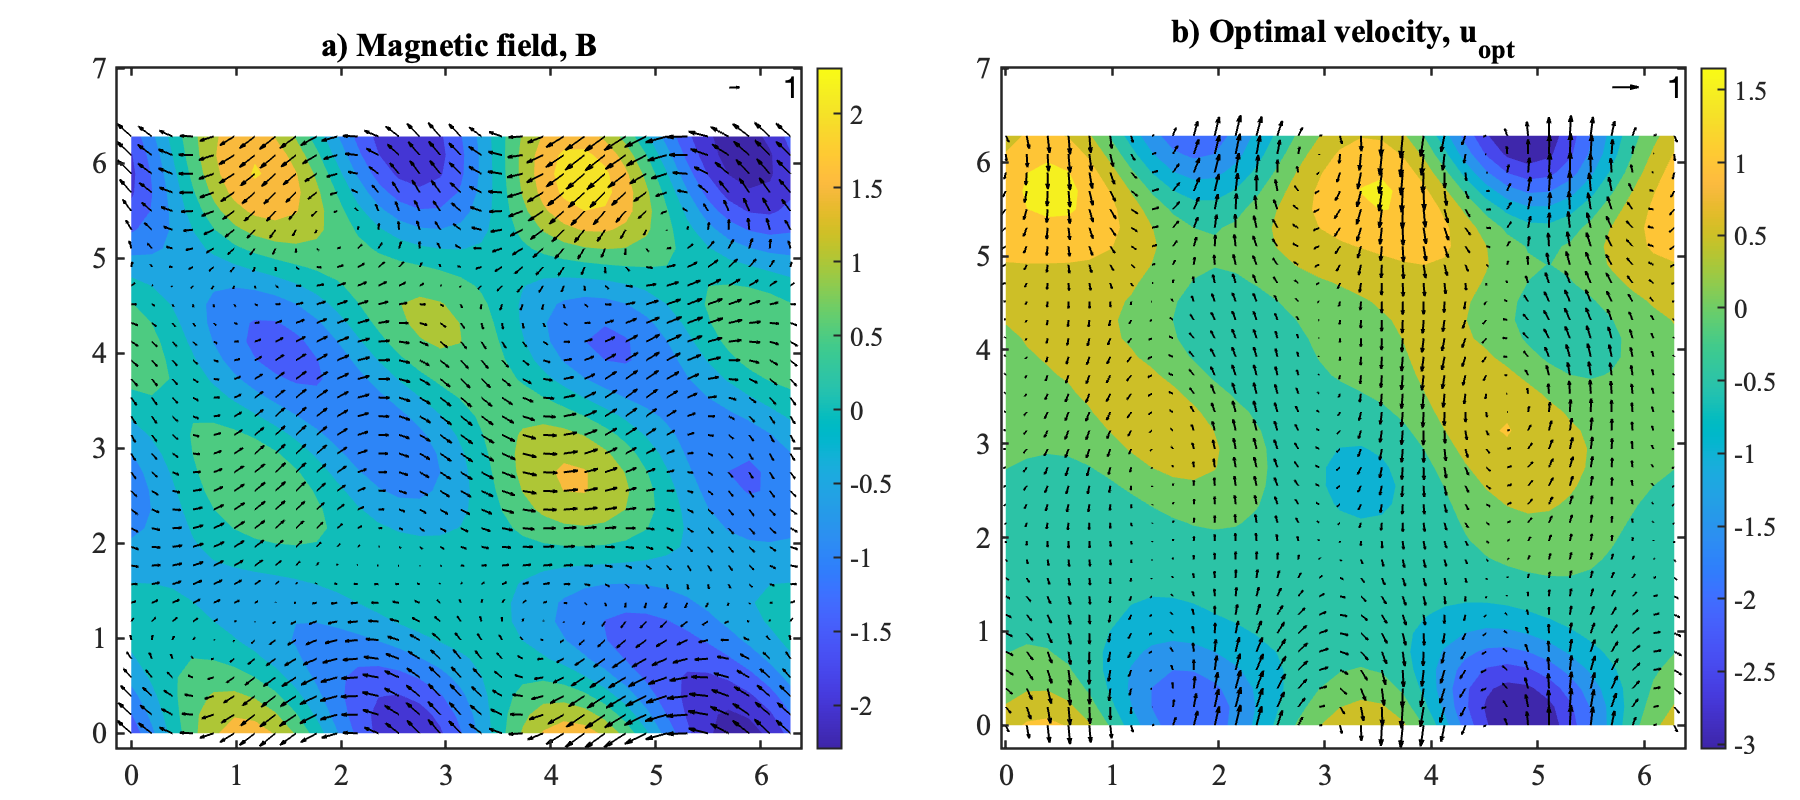
\includegraphics[width=.99 \linewidth]{vfields_opt_K=2.png}
 \caption{
a) $\Bvec$ is optimized for maximal $\dot{M}$ (while using the corresponding $\uopt$ in each iteration of the optimization).
b) The optimal velocity field that corresponds to the optimized $\Bvec$, giving $\dot{M} = 1.53$.}
\label{vfields_opt_K=2}
\end{figure*}
% N =32, K = 2, weight = 0.5



\bibliographystyle{plain}
\bibliography{bib_dynamo}

\end{document}
